\chapter{Multicore Hardware Model}

The computers are used in diverse applications. Applications may provide unique challenge on the way computers process data. For example some application may have one algorithm to be run large amount of data and some others may require large amount of instructions to be executed on small amount of data. These requirements have defined the architecture of computers.
\ifericsson

In this chapter we briefly present the Flynn's taxonomy, discuss about multicore memory models, data sharing concepts and introduce to the Ericsson's DSP multicore platform.
\else

In this chapter we briefly present the Flynn's taxonomy, discuss about multicore memory models and data sharing concepts.

Model and architecture of hardware used for this thesis are intellectual property of Ericsson. This chapter only presents common multicore architectures.
\fi


\section{Computing platforms}

The computing platforms are generally classified based on Flynn's taxonomy \cite{flynn1966very}. The classification is based on number of data and instruction streams. The classification is as follows: 

\begin{enumerate}
\item{Single Instruction Stream-Single Data Stream (SISD)}

A computing unit with single instruction stream and single data stream. For example: single core micro-controllers and micro-processors.

\item{Single Instruction Stream-Multiple Data Stream (SIMD)}

Multiple computing units process same instruction on different data stream. For example: Graphical Processing Units (GPU).

\item{Multiple Instruction Stream-Single Data Stream (MISD)}

Multiple computing units process different instruction on same data. For example fault tolerant systems run different algorithms on same data and analyse the result from both the algorithm.

\item{Multiple Instruction Stream-Multiple Data Stream (MIMD)}.

Multiple instructions streams work on different data. For example, general purpose parallel computers.

\end{enumerate}

Parallel computing makes use of multiple computational units to process data at same time (in parallel) \cite{hennessy2011computer}. The architecture of parallel computers can be SIMD, MISD, MIMD or \emph{heterogeneous architecture}, which is a combination of these architectures.


\section{Multicore Memory models}

The memory model defines the organisation and access mechanisms of computer memory. The memory models are designed to address application specific requirements. The memory models can be classified into Uniformed Memory Access (UMA), Non-Uniform Memory Access, Cache Only Memory Access and Scratchpad Random Memory Access (SRAM).

\subsection{UMA}

In UMA architecture, all the processors share a common main memory and any processor's memory access time to any of the memory region of main memory is independent \cite{hennessy2011computer}.

\subsection{NUMA}

In NUMA architecture, all the processors share a common main memory and access time to a memory region depends on the address space of main memory it is accessing \cite{hennessy2011computer}.

\subsection{COMA}

In COMA architecture, processors do not have a main memory, instead the processors are interconnected and support caches. The data is accessed through caches and \emph{cache coherency} protocol is used.\cite{hagersten1992ddm, hennessy2011computer}

\subsection{SRAM}

In SRAM architecture, all processors support memory blocks supported controlled by programs, called scratchpad memories, as replacement for cache \cite{hennessy2011computer}.

\section{Data sharing}

The parallel programs running in different cores or processors can share data to produce results. Data sharing can be done through sharing memory or through message transfer. In multicore systems, cores are physically near and it is less time consuming to share memory. Any of the above memory models can be used for data sharing. To maintain correctness of data shared by parallel programs, programmers have option of using mutex and \emph{coherency protocols} to keep the data consistent among different cores.

\ifericsson
\section{Ericsson hardware platform}

The platform used for this thesis is a home grown ASIC processor from Ericsson. Platform is designed for \emph{LTE} base stations. The LTE (Long Term Evolution) \index{LTE} is a wireless network standard with high speed data access facilities for mobile phones.

The LTE has large data and instruction parallelism, which has influenced the architecture of the platform. The platform contains multiple cores arranged in heterogeneous architecture with scratchpad memory. \autoref{fig:ericsson:platform} shows the block diagram of platform. The platform contains master cores and slave cores with local scratchpad memory. The cores also share a common scratchpad memory. The master cores are designed to handle incoming radio signals. The master core fetches incoming signal data through peripheral interface. The master cores distribute work computation among slave cores. The slave cores are utilised to accelerate the computation by master cores.



\begin{figure}
\centering
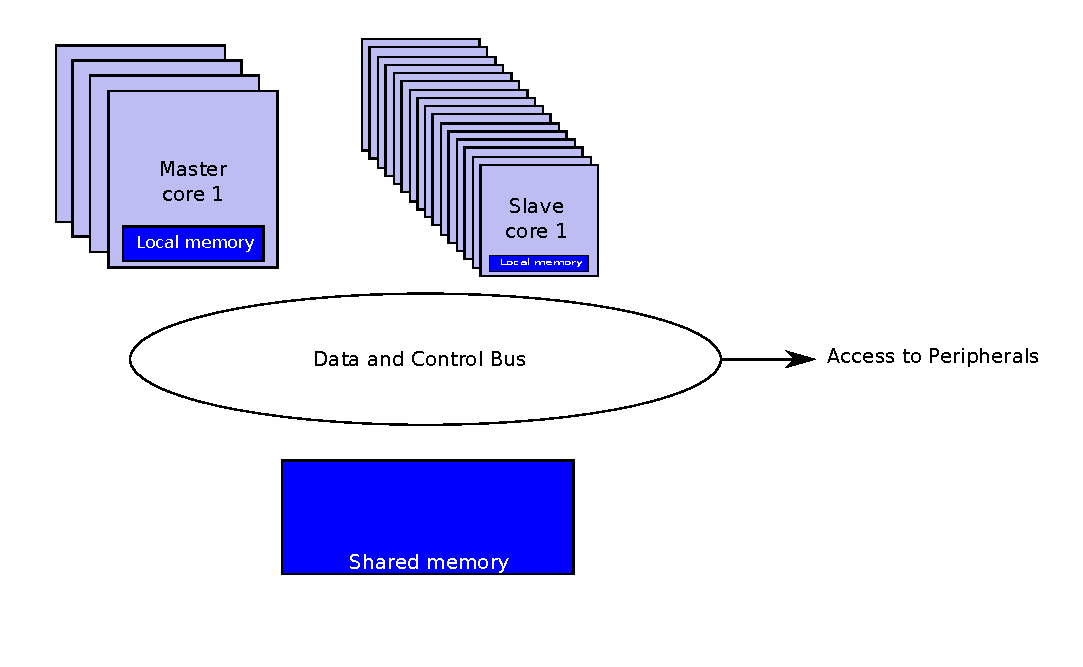
\includegraphics[scale=0.8]{images/EricssonArchitecture.pdf}

    \caption{Ericsson's DSP multicore platform block diagram}
    \label{fig:ericsson:platform}

\end{figure}



\fi





